
\chapter{Radio Scattering}

\section{Scattering Basics, and the $\alpha-4$ Scattering Index}

Scattering causes radiation to follow
different paths through an inhomogeneous plasma. Since
these paths have different lengths, radiation emitted
simultaneously can arrive at different times, broadening
the observed pulse.

We will derive the frequency dependence of this
broadening, assuming a thin scattering screen and
small scattering angles.

\subsubsection{How a Plasma Bends Light}

Recall that the refractive index of a cold plasma is:

\begin{equation}
n=\sqrt{1-\frac{\omega_p^2}{\omega^2}}
\end{equation}

and that $w_p = $, when $w $ we can write:
\begin{equation}
n \simeq 1 -
\frac{n_e e^2}{2\epsilon_0 m_e\omega^2}.
\end{equation}

Therefore,

\begin{equation}
\boxed{n-1\propto n_e\nu^{-2}.}
\end{equation}

If the electron density changes across the wavefront,
different parts of the wave travel at different phase
velocities. This causes the wavefront to rotate, changing
the direction of propagation.

We can derive this using Snell's law.

\begin{equation}
    n_1\sin\phi_1=n_2\sin(\phi_2),
\end{equation}
where $\phi$ is measured relative to the normal of
the boundary.

Consider two adjacent regions with refractive indices
$n$ and $n+dn$. A ray crossing their boundary obeys

\begin{equation}
n\sin\phi=(n+dn)\sin(\phi+d\phi),
\end{equation}



Expanding to first order,

\begin{equation}
n\sin\phi
\simeq n\sin\phi
+dn\sin\phi
+n\cos\phi\,d\phi.
\end{equation}

Rearranging,

\begin{equation}
d\phi=-\frac{\tan\phi}{n}\,dn.
\end{equation}

Now suppose the refractive index varies in the transverse
$x$ direction, while the ray travels approximately along
$z$. For a nearly horizontal refractive-index boundary,
the angle $\phi$ is measured relative to the $x$ direction.

In the small-angle approximation, the ray's angle
relative to $z$ is $\theta=\pi/2-\phi$, so
$d\theta=-d\phi$. Furthermore,

\begin{equation}
\tan\phi \simeq \frac{dz}{dx},
\qquad
dn=\frac{\partial n}{\partial x}\,dx.
\end{equation}

Substituting gives

\begin{equation}
d\theta\simeq
\frac{1}{n}\frac{\partial n}{\partial x}\,dz.
\end{equation}

Since $n\simeq 1$ in a tenuous plasma,

\begin{equation}
\boxed{
\frac{d\theta}{dz}
\simeq \frac{\partial n}{\partial x}.
}
\end{equation}

This is the small-angle ray-bending equation: a
transverse gradient in refractive index changes the
direction of propagation.

\begin{center}
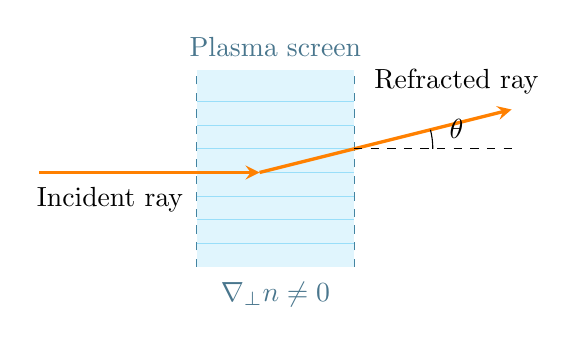
\begin{tikzpicture}[scale=1.0,>=stealth]
    % Plasma screen
    \fill[cyan!12] (2,-1.2) rectangle (4,1.3);
    \draw[cyan!60!black,dashed] (2,-1.2)--(2,1.3);
    \draw[cyan!60!black,dashed] (4,-1.2)--(4,1.3);

    % Density gradient
    \foreach \y in {-0.9,-0.6,...,0.9} {
        \draw[cyan!40] (2,\y)--(4,\y);
    }
    \node[cyan!50!black] at (3,1.6) {Plasma screen};
    \node[cyan!50!black] at (3,-1.55)
        {$\nabla_\perp n\neq 0$};

    % Incoming and outgoing ray
    \draw[very thick,orange,->] (0,0)--(2.8,0);
    \draw[very thick,orange] (2.8,0)--(4,0.3);
    \draw[very thick,orange,->] (4,0.3)--(6,0.8);

    % Reference direction
    \draw[dashed] (4,0.3)--(6,0.3);

    % Angle
    \draw (5,0.3) arc[start angle=0,end angle=14,
                       radius=1];
    \node at (5.3,0.55) {$\theta$};

    \node at (0.9,-0.35) {Incident ray};
    \node at (5.3,1.15) {Refracted ray};
\end{tikzpicture}
\end{center}

For a thin screen, integrate the ray-bending equation
through the plasma:

\begin{equation}
\theta\simeq
\int\frac{\partial n}{\partial x}\,dz.
\end{equation}

Substituting the plasma refractive index,

\begin{equation}
\theta\simeq
-\frac{e^2}{2\epsilon_0m_e\omega^2}
\int\frac{\partial n_e}{\partial x}\,dz.
\end{equation}

Define the electron column density

\begin{equation}
N_e(x)=\int n_e(x,z)\,dz.
\end{equation}

Then

\begin{equation}
\boxed{
\theta\simeq
-\frac{e^2}{2\epsilon_0m_e\omega^2}
\frac{\partial N_e}{\partial x}.
}
\end{equation}

For a fixed transverse electron-density structure,

\begin{equation}
\boxed{\theta\propto\nu^{-2}.}
\end{equation}

Lower-frequency radio waves are therefore deflected
more strongly by the same plasma structure.

\subsubsection{From Scattering Angle to Time Delay}

We now need to determine how much longer a scattered
ray travels compared with an unscattered ray.

Consider a source and observer separated by distance
$D$. A thin scattering screen is located a distance
$D_s$ from the observer.

A ray passes through the screen at transverse
displacement $x$ from the direct line of sight.

\begin{center}
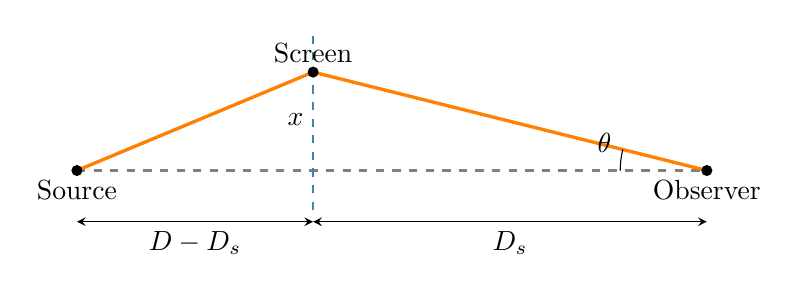
\begin{tikzpicture}[scale=1.0,>=stealth]
    % Coordinates
    \coordinate (S) at (0,0);
    \coordinate (P) at (3,1.25);
    \coordinate (O) at (8,0);

    % Direct path
    \draw[dashed,gray,thick] (S)--(O);

    % Scattered path
    \draw[very thick,orange] (S)--(P)--(O);

    % Screen
    \draw[cyan!60!black,thick,dashed]
        (3,-0.5)--(3,1.8);

    % Points
    \fill (S) circle (2pt);
    \fill (P) circle (2pt);
    \fill (O) circle (2pt);

    % Labels
    \node[below] at (S) {Source};
    \node[below] at (O) {Observer};
    \node[above] at (P) {Screen};
    \node[left] at (3,0.65) {$x$};

    % Distance labels
    \draw[<->] (0,-0.65)--(3,-0.65);
    \node[below] at (1.5,-0.65) {$D-D_s$};

    \draw[<->] (3,-0.65)--(8,-0.65);
    \node[below] at (5.5,-0.65) {$D_s$};

    % Angle at observer
    \draw (6.9,0) arc[start angle=180,
        end angle=166,radius=1.1];
    \node at (6.7,0.35) {$\theta$};
\end{tikzpicture}
\end{center}

Using the Pythagorean theorem, the length of the
scattered path is

\begin{equation}
L_{\rm scatt}
=
\sqrt{(D-D_s)^2+x^2}
+
\sqrt{D_s^2+x^2}.
\end{equation}

The direct path has length

\begin{equation}
L_{\rm direct}=D.
\end{equation}

For small scattering angles, $x\ll D_s$ and
$x\ll D-D_s$. We can use the Taylor expansion

\begin{equation}
\sqrt{a^2+x^2}
=a\sqrt{1+\frac{x^2}{a^2}}
\simeq a+\frac{x^2}{2a}.
\end{equation}

Therefore,

\begin{align}
L_{\rm scatt}
&\simeq (D-D_s)+\frac{x^2}{2(D-D_s)}
+D_s+\frac{x^2}{2D_s}\\
&=D+\frac{x^2}{2}
\left(\frac{1}{D-D_s}+\frac{1}{D_s}\right).
\end{align}

The excess path length is thus

\begin{equation}
\boxed{
\Delta L=
\frac{x^2D}{2D_s(D-D_s)}.
}
\end{equation}

From the geometry, the observed angle between the
scattered ray and the direct line of sight is

\begin{equation}
\theta\simeq\frac{x}{D_s}.
\end{equation}

Substituting $x\simeq D_s\theta$,

\begin{equation}
\boxed{
\Delta L\simeq
\frac{D_sD}{2(D-D_s)}\theta^2.
}
\end{equation}

The additional geometric travel time is
$\tau_{\rm scatt}=\Delta L/c$, giving

\begin{equation}
\boxed{
\tau_{\rm scatt}\simeq
\frac{D_sD}{2c(D-D_s)}\theta^2.
}
\end{equation}

Thus, for a fixed scattering geometry,

\begin{equation}
\boxed{\tau_{\rm scatt}\propto\theta^2.}
\end{equation}

\subsubsection{The Scattering Index}

We have established two relationships:

\begin{equation}
\theta\propto\nu^{-2},
\qquad
\tau_{\rm scatt}\propto\theta^2.
\end{equation}

Combining them,

\begin{equation}
\tau_{\rm scatt}\propto(\nu^{-2})^2.
\end{equation}

Therefore,

\begin{equation}
\boxed{\tau_{\rm scatt}\propto\nu^{-4}.}
\end{equation}

Defining the scattering index $\alpha$ by

\begin{equation}
\tau_{\rm scatt}\propto\nu^\alpha,
\end{equation}

we obtain

\begin{equation}
\boxed{\alpha=-4.}
\end{equation}

This result assumes that the characteristic transverse
plasma structure responsible for deflection is independent
of frequency.

In a turbulent plasma, different frequencies can probe
different spatial scales. For an ideal Kolmogorov
electron-density fluctuation spectrum, the strong-scattering
prediction is instead

\begin{equation}
\boxed{\alpha=-\frac{22}{5}=-4.4.}
\end{equation}
